% Copyright 2005-2016 Airbus-EDF-IMACS-Phimeca
% Permission is granted to copy, distribute and/or modify this document
% under the terms of the GNU Free Documentation License, Version 1.2
% or any later version published by the Free Software Foundation;
% with no Invariant Sections, no Front-Cover Texts, and no Back-Cover
% Texts.  A copy of the license is included in the section entitled "GNU
% Free Documentation License".
\renewcommand{\etapemethodo}{B}
\renewcommand{\nomfichier}{docref_B122_RandomMixture}
\renewcommand{\titrefiche}{Random Mixture : affine combination of independent univariate distributions}

\Header

\MathematicalDescription{

  \underline{\textbf{Goal}}\vspace{2mm}

  A multivariate random variable $\vect{Y}$ may be defined as an affine transform of $n$ independent univariate random variable, as follows :
  \begin{equation}
    \displaystyle \vect{Y}=\vect{y}_0+\mat{M}\,\vect{X}
    \label{RandomMixtureFormula}
  \end{equation}
  where $\vect{y}_0\in\mathbb{R}^d$ is a deterministic vector with $d\in\{1,2,3\}$, $\mat{M}\in\mathcal{M}_{d,n}(\mathbb{R})$ a deterministic matrix and $(X_k)_{ 1 \leq k \leq n}$ are some independent univariate distributions.

  In such a case, it is possible to evaluate directly the distribution of $\vect{Y}$ and then to ask $\vect{Y}$ any request compatible with a distribution : moments, probability and cumulative density functions, quantiles (in dimension 1 only) ...
  \vspace*{2mm}

  \underline{\textbf{Principle}}
  \vspace*{2mm}

  {\bf Evaluation of the probability density  function of the Random Mixture}

  As the univariate random variables $X_i$ are independent, the characteristic function of $\vect{Y}$, denoted $\phi_Y$, is easily defined from the characteristic function of $X_k$ denoted $\phi_{X_k}$ as follows :
  \begin{equation}
    \displaystyle \phi_Y(u_1,\hdots,u_d)=\prod_{j=1}^de^{iu_j{y_0}_j}\prod_{k=1}^n\phi_{X_k}((M^tu)_k), \mbox{  for } \vect{u}\in\mathbb{R}^d
    \label{CharactFuncY}
  \end{equation}

  Once $ \phi_Y$ evaluated, it is possible to evaluate the probability density function of $Y$, denoted $p_Y$ : several techniques are possible, as the inversion of the Fourier transformation. This technique is not easy to implement.\\
  OpenTURNS uses another technique, based on the Poisson sum formulation, defined as follows :
  \begin{equation}
    \displaystyle \sum_{j_1\in\mathbb{Z}}\hdots\sum_{j_d\in\mathbb{Z}} p_Y\left(y_1+\frac{2\pi j_1}{h_1},\hdots,y_d+\frac{2\pi j_d}{h_d}\right)=
    \prod_{j=1}^d \frac{h_j}{2*\pi}\sum_{k_1\in\mathbb{Z}}\hdots\sum_{k_d\in\mathbb{Z}}\phi\left(k_1h_1,\hdots,k_dh_d\right)e^{-\imath(\sum_{m=1}^{d}k_m h_m y_m)}
    \label{PoissonSum}
  \end{equation}
  By fixing $h_1,\hdots,h_d$ small enough, $\frac{2k\pi}{h_j} \approx +\infty$ and $p_Y(\hdots,\frac{2k\pi}{h_j},\hdots) \approx 0$ because of the decreasing properties of $p_Y$.
  Thus the nested sums of the left term of (\ref{PoissonSum}) are reduced to the central term $j_1=\hdots=j_d = 0$~: the left term is approximatively equal to $p_Y(y)$.\\
  Furthermore, the right term of (\ref{PoissonSum}) is a series which converges very fast: only few terms of the series are enough to get machine-precision accuracy. 
  Let us note that the factors $\phi_Y(k_1 h_1,\hdots,k_d,h_d)$, which are expensive to evaluate, do not depend on $y$ and are evaluated once only.\\
  \vspace*{2mm}
  It is also possible to greatly improve the performance of the algorithm by noticing that equation~\eqref{PoissonSum} is linear between $p_Y$
  and $\phi_Y$. We denote $q_Y$ and $\psi_Y$ respectively the density and the characteristic function of the multivariate normal distribution with the
  same mean $\vect{\mu}$ and same covariance matrix $\vect{C}$ as the random mixture. By applying this multivariate normal distribution to the equation~\eqref{PoissonSum}, we obtain by subtraction:
  \begin{equation}
  \displaystyle  p_Y\left(y\right) = \sum_{j\in\mathbb{Z}^d} q_Y\left(y_1+\frac{2\pi j_1}{h_1},\cdots,y_d+\frac{2\pi j_d}{h_d}\right)+
  \frac{H}{2^d\pi^d}\sum_{|k_1|\leq N}\cdots\sum_{|k_d|\leq N} \delta_Y\left(k_1h_1,\cdots,k_dh_d\right)e^{-\imath(\sum_{m=1}^{d}k_m h_m y_m)}
  \label{algoPoisson}
  \end{equation}
  where $H = h_1\times\cdots\times h_d$, $j=(j_1,\cdots,j_d)$, $\delta_Y:=\phi_Y - \psi_Y$\\

  In the case where $n \gg $ 1, using the limit central theorem, the law of $\vect{Y} $ tends to the normal distribution density $q$,
  which will drastically reduce $N$.  The sum on $q$ will become the most CPU-intensive part, because in the general case we will
  have to keep more terms than the central one in this sum, since the parameters $ h_1, \dots  h_d$ were calibrated
  with respect to $p$ and not $q$.

  The parameters $h_1, \dots  h_d$ are calibrated using the following formula:
  \begin{align}
    h_\ell = \frac{2\pi}{(\beta+4\alpha)\sigma_\ell}
  \end{align}
  where $\sigma_\ell=\sqrt{\Cov{\vect{Y}}_{\ell,\ell}}$ and $\alpha$, $\beta$ are respectively the number of standard deviations covered by the marginal distribution
  ($\alpha=5$ by default) and $\beta$ the number of marginal deviations beyond which the density is negligible ($\beta=8.5$ by default).

  The $N$ parameter is dynamically calibrated: we start with $N=8$ then we double $N$ value until the total contribution of the additional terms is negligible.

  \vspace*{2mm}

  {\bf Evaluation of the moments of the Random Mixture}

  The relation (\ref{RandomMixtureFormula}) enables to evaluate all the moments of the random mixture, if mathematically defined. For example, we have :
  \begin{align*}
    \left\{
    \begin{array}{lcl}
      \Expect{\vect{Y}} & = & \vect{y_0} + \mat{M}\Expect{\vect{X}} \\
      \Cov{\vect{Y}} & = & \mat{M}\,\Cov{\vect{X}}\mat{M}^t
    \end{array}
    \right.
  \end{align*}
  \vspace*{2mm}
  
  {\bf Computation on a regular grid}

  The interest is to compute the density function on a regular grid. Purposes are to get quickly ann approximation.
  The regular grid is of form:
  \begin{align}
    \forall r\in\{1,\hdots,d\},\forall m\in\{0,\hdots,M-1\},\:y_{r,m}=\mu_r+b\left(\frac{2m+1}{M} - 1\right)\sigma_r
  \end{align}

  By denoting $p_{m_1,\hdots,m_d}=p_{\vect{Y}}(y_{1,m_1},\hdots,y_{d,m_d})$:
  \begin{align}
    p_{m_1,\hdots,m_d}= Q_{m_1,\hdots,m_d}+S_{m_1,\hdots,m_d}
  \end{align}
  for which the term $S_{m_1,\hdots,m_d}$ is the most CPU consuming. This term rewrites:
  \begin{align}
  S_{m_1,\hdots,m_d}=&\frac{H}{2^d\pi^d}\sum_{k_1=-N}^{N}\hdots\sum_{k_d=-N}^{N}\delta\left(k_1h_1,\hdots,k_dh_d\right)
  E_{m_1,\hdots,m_d}(k_1,\hdots,k_d) \label{Eq:S}
  \end{align}
  with:
  \begin{align}
    \delta\left(k_1h_1,\hdots,k_dh_d\right)&=(\phi-\psi)\left(k_1h_1,\hdots,k_dh_d\right)\\
    E_{m_1,\hdots,m_d}(k_1,\hdots,k_d)&=e^{-i\sum_{j=1}^d k_jh_j\left(\mu_j+b\left(\frac{2m_j+1}{M}-1\right)\sigma_j\right)}
  \end{align}

  The aim is to rewrite the previous expression as a $d$- discrete Fourier transform, in order to apply Fast Fourier Transform (\emph{FFT}) for its evaluation.

  We set $M=N$ and $\forall j \in\{1,\hdots,d\},\: h_j=\frac{\pi}{b\sigma_j}$ and $\tau_j=\frac{\mu_j}{b\sigma_j}$.
  For convenience, we introduce the functions:
  $$
  f_j(k) = e^{-i\pi (k+1)\left(\tau_j-1+\frac{1}{N}\right)}
  $$
  We use $k+1$ instead of $k$ in this function to simplify expressions below.

  We obtain:
  \begin{align}
  E_{m_1,\hdots,m_d}(k_1,\hdots,k_d)&=e^{-i\sum_{j=1}^{d} k_jh_jb\sigma_j\left(\frac{\mu_j}{b\sigma_j}+\frac{2m_j}{N}+\frac{1}{N}-1\right)}\notag\\
    &=e^{-2i\pi\left(\frac{\sum_{j=1}^{d}k_j m_j}{N}\right)}e^{-i\pi\sum_{j=1}^{d} k_j\left(\tau_j-1+\frac{1}{N}\right)} \notag\\
    &=e^{-2i\pi\left(\frac{\sum_{j=1}^{d}k_j m_j}{N}\right)} f_1(k_1-1) \times\hdots\times f_d(k_d-1) \label{Eq:E}
  \end{align}

  For performance reasons, we want to use the discrete Fourier transform with the following convention in dimension 1~:
  $$
  A_m = \sum_{k=0}^{N-1} a_k e^{-2i\pi\frac{km}{N}}
  $$
  which extension to dimensions 2 and 3 are respectively~:
  $$
  A_{m,n} = \sum_{k=0}^{N-1}\sum_{l=0}^{N-1} a_{k,l} e^{-2i\pi\frac{km}{N}} e^{-2i\pi\frac{ln}{N}}\\
  $$

  $$
  A_{m,n,p} = \sum_{k=0}^{N-1}\sum_{l=0}^{N-1}\sum_{s=0}^{N-1} a_{k,l,s} e^{-2i\pi\frac{km}{N}} e^{-2i\pi\frac{ln}{N}} e^{-2i\pi\frac{sp}{N}}
  $$

  We decompose sums of~\eqref{Eq:S} on the interval $[-N,N]$ into three parts:
  \begin{align}
  \sum_{k_j=-N}^{N}\delta\left(k_1h_1,\hdots,k_dh_d\right) E_{m_1,\hdots,m_d}(k_1,\hdots,k_d)
    = & \sum_{k_j=-N}^{-1} \delta\left(k_1h_1,\hdots,k_dh_d\right) E_{m_1,\hdots,m_d}(k_1,\hdots,k_d) \notag\\
    & + \delta\left(k_1h_1,\hdots,0,\hdots,k_dh_d\right) E_{m_1,\hdots,0,\hdots,m_d}(k_1,\hdots,0,\hdots,k_d) \notag\\
    & + \sum_{k_j=1}^{N}\delta\left(k_1h_1,\hdots,k_dh_d\right) E_{m_1,\hdots,m_d}(k_1,\hdots,k_d) \label{Eq:decomposition-sum}
  \end{align}

  If we already computed $E$ for dimension $d-1$, then the middle term in this sum is trivial.

  To compute the last sum of~\eqref{Eq:decomposition-sum}, we apply a change of variable $k_j'=k_j-1$:
  \begin{align}
  \sum_{k_j=1}^{N}\delta\left(k_1h_1,\hdots,k_dh_d\right) E_{m_1,\hdots,m_d}(k_1,\hdots,k_d)
  = & \sum_{k_j=0}^{N-1}\delta\left(k_1h_1,\hdots,(k_j+1)h_j,\hdots,k_dh_d\right) \times\notag\\
    & \hspace*{3cm} E_{m_1,\hdots,m_d}(k_1,\hdots,k_j+1,\hdots,k_d)
  \end{align}
  Equation~\eqref{Eq:E} gives:
  \begin{align}
  E_{m_1,\hdots,m_d}(k_1,\hdots,k_j+1,\hdots,k_d) 
  &= 
      e^{-2i\pi\left(\frac{\sum_{l=1}^{d}k_l m_l}{N} +\frac{m_j}{N}\right)}
      f_1(k_1-1)\times\hdots\times f_j(k_j)\times\hdots\times f_d(k_d-1)\notag\\
  &= 
      e^{-2i\pi\left(\frac{m_j}{N}\right)}
      e^{-2i\pi\left(\frac{\sum_{l=1}^{d}k_l m_l}{N}\right)}
      f_1(k_1-1)\times\hdots\times f_j(k_j)\times\hdots\times f_d(k_d-1)
  \end{align}
  Thus
  \begin{align}
  \sum_{k_j=1}^{N}\delta\left(k_1h_1,\hdots,k_dh_d\right) E_{m_1,\hdots,m_d}&(k_1,\hdots,k_d)
    = e^{-2i\pi\left(\frac{m_j}{N}\right)} \sum_{k_j=0}^{N-1}\delta\left(k_1h_1,\hdots,(k_j+1)h_j,\hdots,k_dh_d\right) \times\notag\\
    & e^{-2i\pi\left(\frac{\sum_{l=1}^{d}k_l m_l}{N}\right)}
      f_1(k_1-1)\times\hdots\times f_j(k_j)\times\hdots\times f_d(k_d-1) \label{Eq:j-sigma+}
  \end{align}

  To compute the first sum of equation~\eqref{Eq:decomposition-sum}, we apply a change of variable $k_j'=N+k_j$:
  \begin{align}
  \sum_{k_j=-N}^{-1}\delta\left(k_1h_1,\hdots,k_dh_d\right) E_{m_1,\hdots,m_d}(k_1,\hdots,k_d)
  = & \sum_{k_j=0}^{N-1}\delta\left(k_1h_1,\hdots,(k_j-N)h_j,\hdots,k_dh_d\right) \times\notag\\
    & \hspace*{3cm} E_{m_1,\hdots,m_d}(k_1,\hdots,k_j-N,\hdots,k_d)
  \end{align}
  Equation~\eqref{Eq:E} gives:
  \begin{align}
  E_{m_1,\hdots,m_d}(k_1,\hdots,k_j-N,\hdots,k_d) 
  &= 
      e^{-2i\pi\left(\frac{\sum_{l=1}^{d}k_l m_l}{N} -m_j\right)}
      f_1(k_1-1)\times\hdots\times f_j(k_j-1-N)\times\hdots\times f_d(k_d-1) \notag\\
  &= 
      e^{-2i\pi\left(\frac{\sum_{l=1}^{d}k_l m_l}{N}\right)}
      f_1(k_1-1)\times\hdots\times \overline{f}_j(N-1-k_j)\times\hdots\times f_d(k_d-1) 
  \end{align}

  Thus:
  \begin{align}
  \sum_{k_j=-N}^{-1}\delta\left(k_1h_1,\hdots,k_dh_d\right) E_{m_1,\hdots,m_d}&(k_1,\hdots,k_d)
    = \sum_{k_j=0}^{N-1}\delta\left(k_1h_1,\hdots,(k_j-N)h_j,\hdots,k_dh_d\right) \times\notag\\
    & e^{-2i\pi\left(\frac{\sum_{l=1}^{d}k_l m_l}{N}\right)}
      f_1(k_1-1)\times\hdots\times \overline{f}_j(N-1-k_j)\times\hdots\times f_d(k_d-1) \label{Eq:j-sigma-}
  \end{align}

  To summarize:
  \begin{enumerate}
  \item In order to compute sum from $k_1=1$ to $N$, we multiply by $e^{-2i\pi\left(\frac{m_1}{N}\right)}$ and consider $\delta((k_1+1)h,\hdots)f_1(k_1)$
  \item In order to compute sum from $k_1=-N$ to $-1$, we consider $\delta((k_1-N)h,\hdots)\overline{f}_1(N-1-k_1)$
  \end{enumerate}
  
  

  {\bf OpenTURNS}\\
  In the 0.13 version of OpenTURNS, distributions which are able to evaluate their characteristic function are the following ones :  $\chi^2$, Exponential, Gamma,  Laplace, Logistic, Mixture, univariate Normal, Rayleigh, Triangular, univariate TruncatedNormal, Uniform, KernelMixture (which the distribution coming from a kernel smoothing method without treatment of bounds), RandomMixture.\\
  Thus, all the requests to $Y$ that require the evaluation of the probability density function may be satisfied only if the univariate random variables $X_i$ follow distributions which characteristic function has been implemented.\\

  Until the 1.5 version of OpenTURNS, only univariate random mixtures were available.
  For all the other requests, no restriction is assigned.
}
{
  --
}


\Methodology{
  Within the global methodology, random mixtures may be used to define the output variable of interest from some indepedent univariate random variables, within the step B.
}
            {
                "Abate, J. and Whitt, W. (1992). The Fourier-series method for inverting transforms of probability distributions. Queueing Systems 10, 5--88., 1992", formula 5.5.
            }


            \Example{
              The example here is an output variable of interest defined as the following combination :
              \begin{align*}
                Y = 2 + 5X_1 + X_2
              \end{align*}
              where $X_1$ and $X_2$ are independent and :
              \begin{itemize}
              \item  $X_1$ follows a $\cE(1.5)$,
              \item  $X_2$ follows a $\cN(4,1)$.
              \end{itemize}

              The pdf and cdf graphs are the following ones.

              \begin{center}
                \begin{tabular}{cc}
                  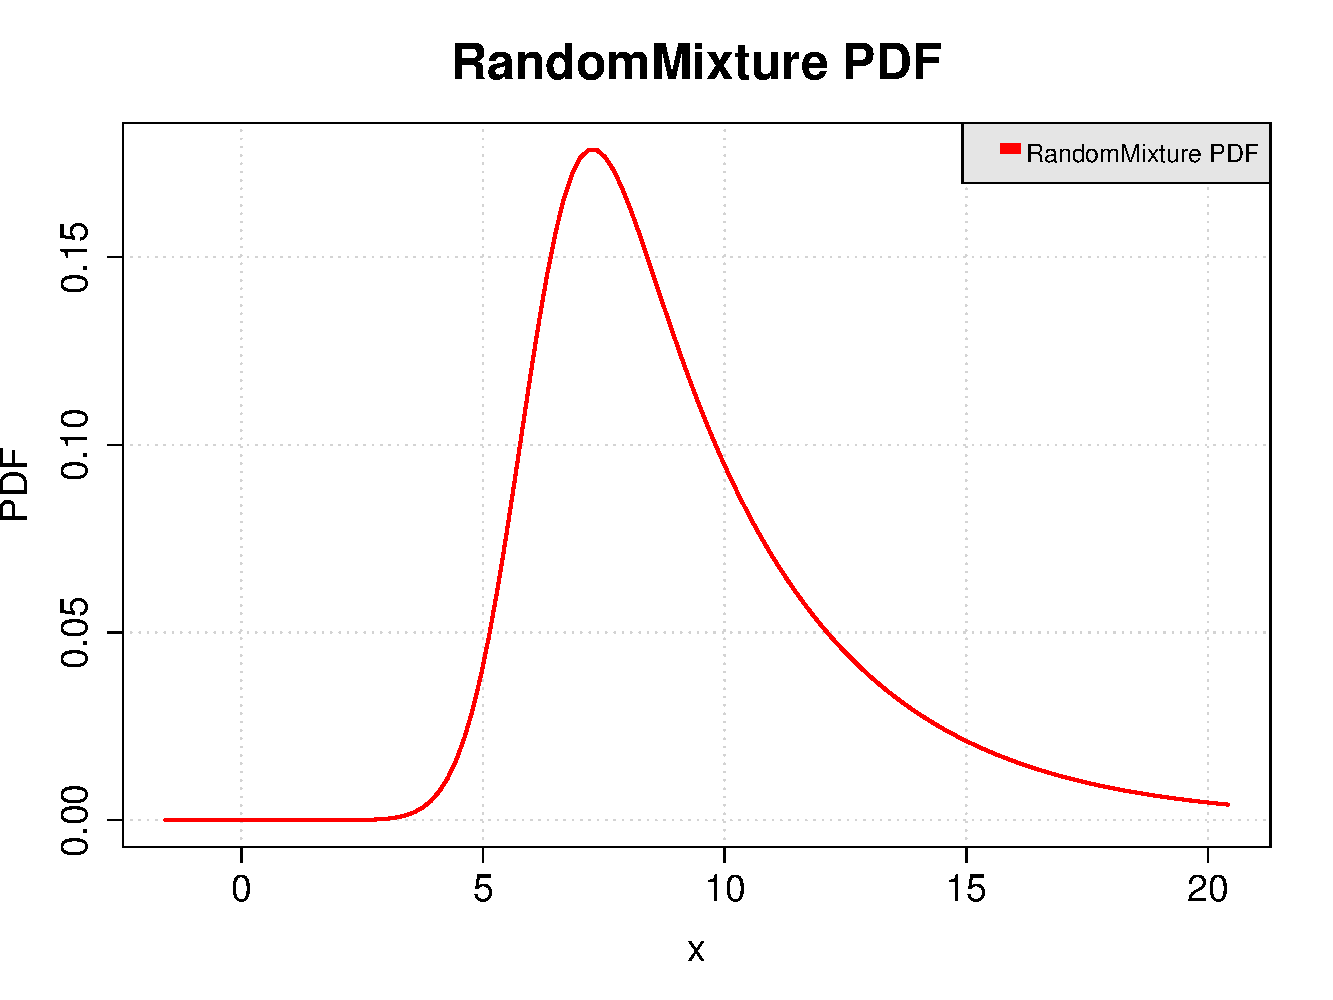
\includegraphics[width=8cm]{Figures/RandomMixture_pdf.pdf} &   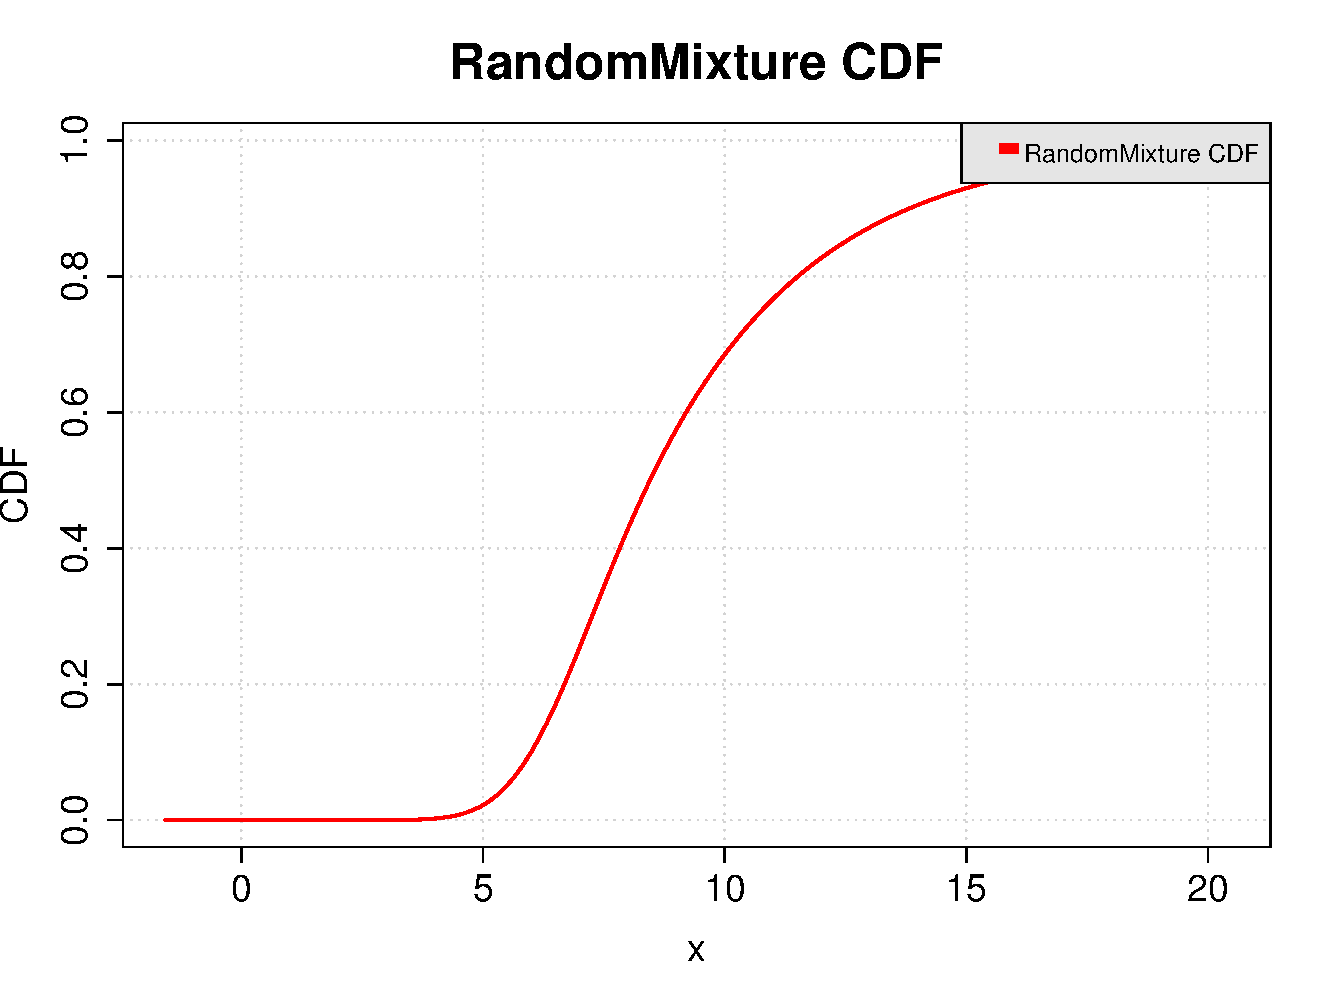
\includegraphics[width=8cm]{Figures/RandomMixture_cdf.pdf}
                \end{tabular}
              \end{center}





            }
